% $Id$
\documentclass{article}

\usepackage{ifpdf}
\usepackage{graphicx}
\usepackage[dutch]{babel}
\usepackage{listings}

% @(#)$Id: jml-listings.tex,v 1.4 2006/09/02 17:06:31 leavens Exp $
%
% Copyright (C) 2006 Iowa State University
%
% This file is part of JML
%
% JML is free software; you can redistribute it and/or modify
% it under the terms of the GNU General Public License as published by
% the Free Software Foundation; either version 2, or (at your option)
% any later version.
%
% JML is distributed in the hope that it will be useful,
% but WITHOUT ANY WARRANTY; without even the implied warranty of
% MERCHANTABILITY or FITNESS FOR A PARTICULAR PURPOSE.  See the
% GNU General Public License for more details.
%
% You should have received a copy of the GNU General Public License
% along with JML; see the file COPYING.  If not, write to
% the Free Software Foundation, 675 Mass Ave, Cambridge, MA 02139, USA.
%
% A JML listings environment.
%
% AUTHOR: Gary T. Leavens
%
% requires listings i.e., do \usepackage{listings} first
%
% This file is set up to be used via % @(#)$Id: jml-listings.tex,v 1.4 2006/09/02 17:06:31 leavens Exp $
%
% Copyright (C) 2006 Iowa State University
%
% This file is part of JML
%
% JML is free software; you can redistribute it and/or modify
% it under the terms of the GNU General Public License as published by
% the Free Software Foundation; either version 2, or (at your option)
% any later version.
%
% JML is distributed in the hope that it will be useful,
% but WITHOUT ANY WARRANTY; without even the implied warranty of
% MERCHANTABILITY or FITNESS FOR A PARTICULAR PURPOSE.  See the
% GNU General Public License for more details.
%
% You should have received a copy of the GNU General Public License
% along with JML; see the file COPYING.  If not, write to
% the Free Software Foundation, 675 Mass Ave, Cambridge, MA 02139, USA.
%
% A JML listings environment.
%
% AUTHOR: Gary T. Leavens
%
% requires listings i.e., do \usepackage{listings} first
%
% This file is set up to be used via % @(#)$Id: jml-listings.tex,v 1.4 2006/09/02 17:06:31 leavens Exp $
%
% Copyright (C) 2006 Iowa State University
%
% This file is part of JML
%
% JML is free software; you can redistribute it and/or modify
% it under the terms of the GNU General Public License as published by
% the Free Software Foundation; either version 2, or (at your option)
% any later version.
%
% JML is distributed in the hope that it will be useful,
% but WITHOUT ANY WARRANTY; without even the implied warranty of
% MERCHANTABILITY or FITNESS FOR A PARTICULAR PURPOSE.  See the
% GNU General Public License for more details.
%
% You should have received a copy of the GNU General Public License
% along with JML; see the file COPYING.  If not, write to
% the Free Software Foundation, 675 Mass Ave, Cambridge, MA 02139, USA.
%
% A JML listings environment.
%
% AUTHOR: Gary T. Leavens
%
% requires listings i.e., do \usepackage{listings} first
%
% This file is set up to be used via \input{jml-listings}.
% If you want, you could make a version that is a style file,
% but then change \lstdefinelanguage to \lst@definelanguage below.
%
\lstdefinelanguage[JML]{Java}[]{Java}%
       {% C++ style comments have to start with a blank!
        comment=[l]{//\ },
        % And C-style comments must also start with a blank!
        morecomment=[s]{/*\ }{*/},
        % sensitive=true, % inherited
        % Add JML keywords as level 1 keywords, so can typeset differently
        classoffset=1,
        % And here are all the wonderful JML keywords
        morekeywords={abrupt_behavior,abrupt_behaviour,
         accessible,accessible_redundantly,also,assert,assert_redundantly,
         assignable,assignable_redundantly,assume,assume_redundantly,
         axiom,behavior,behaviour,breaks,breaks_redundantly,
         callable,callable_redundantly,captures,captures_redundantly,
         choose,choose_if,code,code_bigint_math,code_java_math,
         code_safe_math,constraint,constraint_redundantly,constructor,
         continues,continues_redundantly,decreases,decreases_redundantly,
         decreasing,decreasing_redundantly,diverges,diverges_redundantly,
         duration,duration_redundantly,ensures,ensures_redundantly,
         example,exceptional_behavior,exceptional_behaviour,
         exceptional_example,exsures,exsures_redundantly,field,
         forall,for_example,ghost,helper,hence_by,hence_by_redundantly,
         implies_that,in,in_redundantly,initializer,initially,instance,
         invariant,invariant_redundantly,loop_invariant,
         loop_invariant_redundantly,maintaining,maintaining_redundantly,
         maps,maps_redundantly,measured_by,measured_by_redundantly,method,
         model,model_program,modifiable,modifiable_redundantly,modifies,
         modifies_redundantly,monitored,monitors_for,non_null,
         normal_behavior,normal_behaviour,normal_example,nowarn,
         nullable,nullable_by_default,old,or,post,post_redundantly,
         pre,pre_redundantly,pure,readable,refine,refines,represents,
         represents_redundantly,requires,requires_redundantly,
         returns,returns_redundantly,set,signals,signals_only,
         signals_only_redundantly,signals_redundantly,spec_bigint_math,
         spec_java_math,spec_protected,spec_public,spec_safe_math,
         static_initializer,uninitialized,unreachable,weakly,
         when,when_redundantly,working_space,working_space_redundantly,
         writable
        },
        % keywords from the universe type system
        morekeywords={rep,peer,readonly},
        % typeset everything that starts with a backslash as a keyword
        % BUG: this doesn't allow typesetting these keywords differently
        keywordsprefix=\\,
        otherkeywords={<:,<-,->,..,<==,==>,<==>,<=!=>},
        classoffset=0 % restore default class for keywords
}
.
% If you want, you could make a version that is a style file,
% but then change \lstdefinelanguage to \lst@definelanguage below.
%
\lstdefinelanguage[JML]{Java}[]{Java}%
       {% C++ style comments have to start with a blank!
        comment=[l]{//\ },
        % And C-style comments must also start with a blank!
        morecomment=[s]{/*\ }{*/},
        % sensitive=true, % inherited
        % Add JML keywords as level 1 keywords, so can typeset differently
        classoffset=1,
        % And here are all the wonderful JML keywords
        morekeywords={abrupt_behavior,abrupt_behaviour,
         accessible,accessible_redundantly,also,assert,assert_redundantly,
         assignable,assignable_redundantly,assume,assume_redundantly,
         axiom,behavior,behaviour,breaks,breaks_redundantly,
         callable,callable_redundantly,captures,captures_redundantly,
         choose,choose_if,code,code_bigint_math,code_java_math,
         code_safe_math,constraint,constraint_redundantly,constructor,
         continues,continues_redundantly,decreases,decreases_redundantly,
         decreasing,decreasing_redundantly,diverges,diverges_redundantly,
         duration,duration_redundantly,ensures,ensures_redundantly,
         example,exceptional_behavior,exceptional_behaviour,
         exceptional_example,exsures,exsures_redundantly,field,
         forall,for_example,ghost,helper,hence_by,hence_by_redundantly,
         implies_that,in,in_redundantly,initializer,initially,instance,
         invariant,invariant_redundantly,loop_invariant,
         loop_invariant_redundantly,maintaining,maintaining_redundantly,
         maps,maps_redundantly,measured_by,measured_by_redundantly,method,
         model,model_program,modifiable,modifiable_redundantly,modifies,
         modifies_redundantly,monitored,monitors_for,non_null,
         normal_behavior,normal_behaviour,normal_example,nowarn,
         nullable,nullable_by_default,old,or,post,post_redundantly,
         pre,pre_redundantly,pure,readable,refine,refines,represents,
         represents_redundantly,requires,requires_redundantly,
         returns,returns_redundantly,set,signals,signals_only,
         signals_only_redundantly,signals_redundantly,spec_bigint_math,
         spec_java_math,spec_protected,spec_public,spec_safe_math,
         static_initializer,uninitialized,unreachable,weakly,
         when,when_redundantly,working_space,working_space_redundantly,
         writable
        },
        % keywords from the universe type system
        morekeywords={rep,peer,readonly},
        % typeset everything that starts with a backslash as a keyword
        % BUG: this doesn't allow typesetting these keywords differently
        keywordsprefix=\\,
        otherkeywords={<:,<-,->,..,<==,==>,<==>,<=!=>},
        classoffset=0 % restore default class for keywords
}
.
% If you want, you could make a version that is a style file,
% but then change \lstdefinelanguage to \lst@definelanguage below.
%
\lstdefinelanguage[JML]{Java}[]{Java}%
       {% C++ style comments have to start with a blank!
        comment=[l]{//\ },
        % And C-style comments must also start with a blank!
        morecomment=[s]{/*\ }{*/},
        % sensitive=true, % inherited
        % Add JML keywords as level 1 keywords, so can typeset differently
        classoffset=1,
        % And here are all the wonderful JML keywords
        morekeywords={abrupt_behavior,abrupt_behaviour,
         accessible,accessible_redundantly,also,assert,assert_redundantly,
         assignable,assignable_redundantly,assume,assume_redundantly,
         axiom,behavior,behaviour,breaks,breaks_redundantly,
         callable,callable_redundantly,captures,captures_redundantly,
         choose,choose_if,code,code_bigint_math,code_java_math,
         code_safe_math,constraint,constraint_redundantly,constructor,
         continues,continues_redundantly,decreases,decreases_redundantly,
         decreasing,decreasing_redundantly,diverges,diverges_redundantly,
         duration,duration_redundantly,ensures,ensures_redundantly,
         example,exceptional_behavior,exceptional_behaviour,
         exceptional_example,exsures,exsures_redundantly,field,
         forall,for_example,ghost,helper,hence_by,hence_by_redundantly,
         implies_that,in,in_redundantly,initializer,initially,instance,
         invariant,invariant_redundantly,loop_invariant,
         loop_invariant_redundantly,maintaining,maintaining_redundantly,
         maps,maps_redundantly,measured_by,measured_by_redundantly,method,
         model,model_program,modifiable,modifiable_redundantly,modifies,
         modifies_redundantly,monitored,monitors_for,non_null,
         normal_behavior,normal_behaviour,normal_example,nowarn,
         nullable,nullable_by_default,old,or,post,post_redundantly,
         pre,pre_redundantly,pure,readable,refine,refines,represents,
         represents_redundantly,requires,requires_redundantly,
         returns,returns_redundantly,set,signals,signals_only,
         signals_only_redundantly,signals_redundantly,spec_bigint_math,
         spec_java_math,spec_protected,spec_public,spec_safe_math,
         static_initializer,uninitialized,unreachable,weakly,
         when,when_redundantly,working_space,working_space_redundantly,
         writable
        },
        % keywords from the universe type system
        morekeywords={rep,peer,readonly},
        % typeset everything that starts with a backslash as a keyword
        % BUG: this doesn't allow typesetting these keywords differently
        keywordsprefix=\\,
        otherkeywords={<:,<-,->,..,<==,==>,<==>,<=!=>},
        classoffset=0 % restore default class for keywords
}

%\lstset{language=[jml]java}
\lstset{breaklines}
\lstset{tabsize=2}
\lstset{stepnumber=0}
\lstset{basicstyle=\scriptsize}
\lstset{escapechar=\#}
\lstset{flexiblecolumns}
\lstset{frame=tb}


\author{Hubbers \and Jacobs \and Kiniry \and Oostdijk}
\title{Formele methoden bij internet stemming}

\begin{document}
\maketitle

\section{Formele methoden bij het KOA project}
KOA staat voor Kiezen Op Afstand en wordt gebruikt om een proef om via
internet te stemmen mee aan te duiden.
Deze proef is specifiek opgezet voor de Europese verkiezingen in juni 2004.

De Security of Systems groep van de KUN is actief betrokken bij dit project.
In 2003 heeft zij 
een blackbox test uitgevoerd op het gebied van netwerk en systeem test.
Verder heeft zij
zitting gehad in een panel van experts. E\'en van de aanbevelingen van dit panel betrof het inhuren van een onafhankelijke derde partij die de uitslag van
de verkiezingen moet kunnen controleren.
Deze aanbeveling is overgenomen door het ministerie. De SoS groep heeft hierop
een offerte ingediend waarbij de nadruk is gelegd op het gebruik van formele methoden om zo'n hertelapplicatie te schrijven.
Enigszins tot onze verrassing bleken wij de aanbestedingsronde te hebben 
gewonnen. Uit communicatie met het ministerie bleek dat zij bewust hebben 
gekozen voor deze formele methoden om de vertrouwensbasis in het programma
te vergroten.

De applicatie is geschreven in Java. De specificaties zijn geschreven in JML, 
de Java Modeling Language.
Deze taal wordt steeds vaker gebruikt om correctheid van Java programma's
mee te bewijzen. Die populariteit is mede te danken aan de hoeveelheid
beschikbare tools die gebruikt kunnen worden. Vari\"erend van volledige
verificatie tot runtime assertion checking, is er voor elk doel wel
een tool beschikbaar.
Wegens het gebrek aan tijd voor dit project, is hier gekozen voor het gebruik van automatische tools: de runtime assertion checker JMLRAC en de statische checker ESC/Java2. 

Maar deze tools doen natuurlijk nog niets als er geen specificaties worden
geschreven. Wij hebben geprobeerd ons zo goed mogelijk te houden aan het
principe van eerst de specificatie schrijven en daarna pas de implementatie.
Echter, wij moeten bekennen dat dat ons niet consequent gelukt is. De verleiding
om snel te zien of een bepaalde methode daadwerkelijk met de gegeven testfiles
om kan gaan is vaak te groot gebleken.
Wij hebben echter wel ons best gedaan om achteraf zoveel mogelijk specificaties
toe te voegen.

Zoals gebruikelijk was ook deze hertelapplicatie goed op te delen in
verschillende modules. Een module voor de user interface, een module voor
file I/O en natuurlijk de harde kern waar de gegevens worden opgeslagen en
de uitslag van de stemming bepaald.
Voor wat betreft de specificaties hebben wij ervoor gekozen de nadruk te 
leggen op de kern van het systeem: die moest zo volledig mogelijk gespecificeerd
en geverifieerd worden. De andere twee modules zijn minder gedetailleerd
gespecificeerd. In tabel~\ref{tab:locs} is de verhouding tussen de regels
code en specificaties te zien zoals die met de JavaNCSS tool zijn bepaald.
\begin{table}[htbp]
  \caption{KOA specificatie/implementatie verhouding}
  \label{tab:locs}
  \begin{center}
    \begin{tabular}{|l|ccc|}
      \hline
      \quad     & \textbf{File I/O} & \textbf{GUI} & \textbf{Kern} \\
      \hline
       aantal klassen & 8                 & 13                     & 6             \\
       aantal methodes & 154               & 200                    & 83            \\
      aantal regels code      & 837               & 1,599                  & 395           \\
      aantal regels specificatie     & 446               & 172                    & 529           \\
      specificatie:implementatie verhouding & 1:2              & 1:10                   & 5:4           \\
      \hline
    \end{tabular}
  \end{center}
\end{table}

Nu getoond is hoeveel er ongeveer gespecificeerd is, is de volgende vraag
natuurlijk wat er dan zoal gespecificeerd is.
Hiervoor kijken we eerst naar het GUI gedeelte.
De GUI was nagenoeg geheel vastgelegd door het ministerie. Het zou een simpele reeks knoppen moeten worden waarbij het vooral belangrijk was dat men de 
verschillende functies niet in een verkeerde volgorde kan aanroepen.
Zie figuur~\ref{fig:gui} voor een screenshot van het hoofdmenu van de GUI.
\begin{figure}[htb]
  \begin{center}
    \ifpdf
    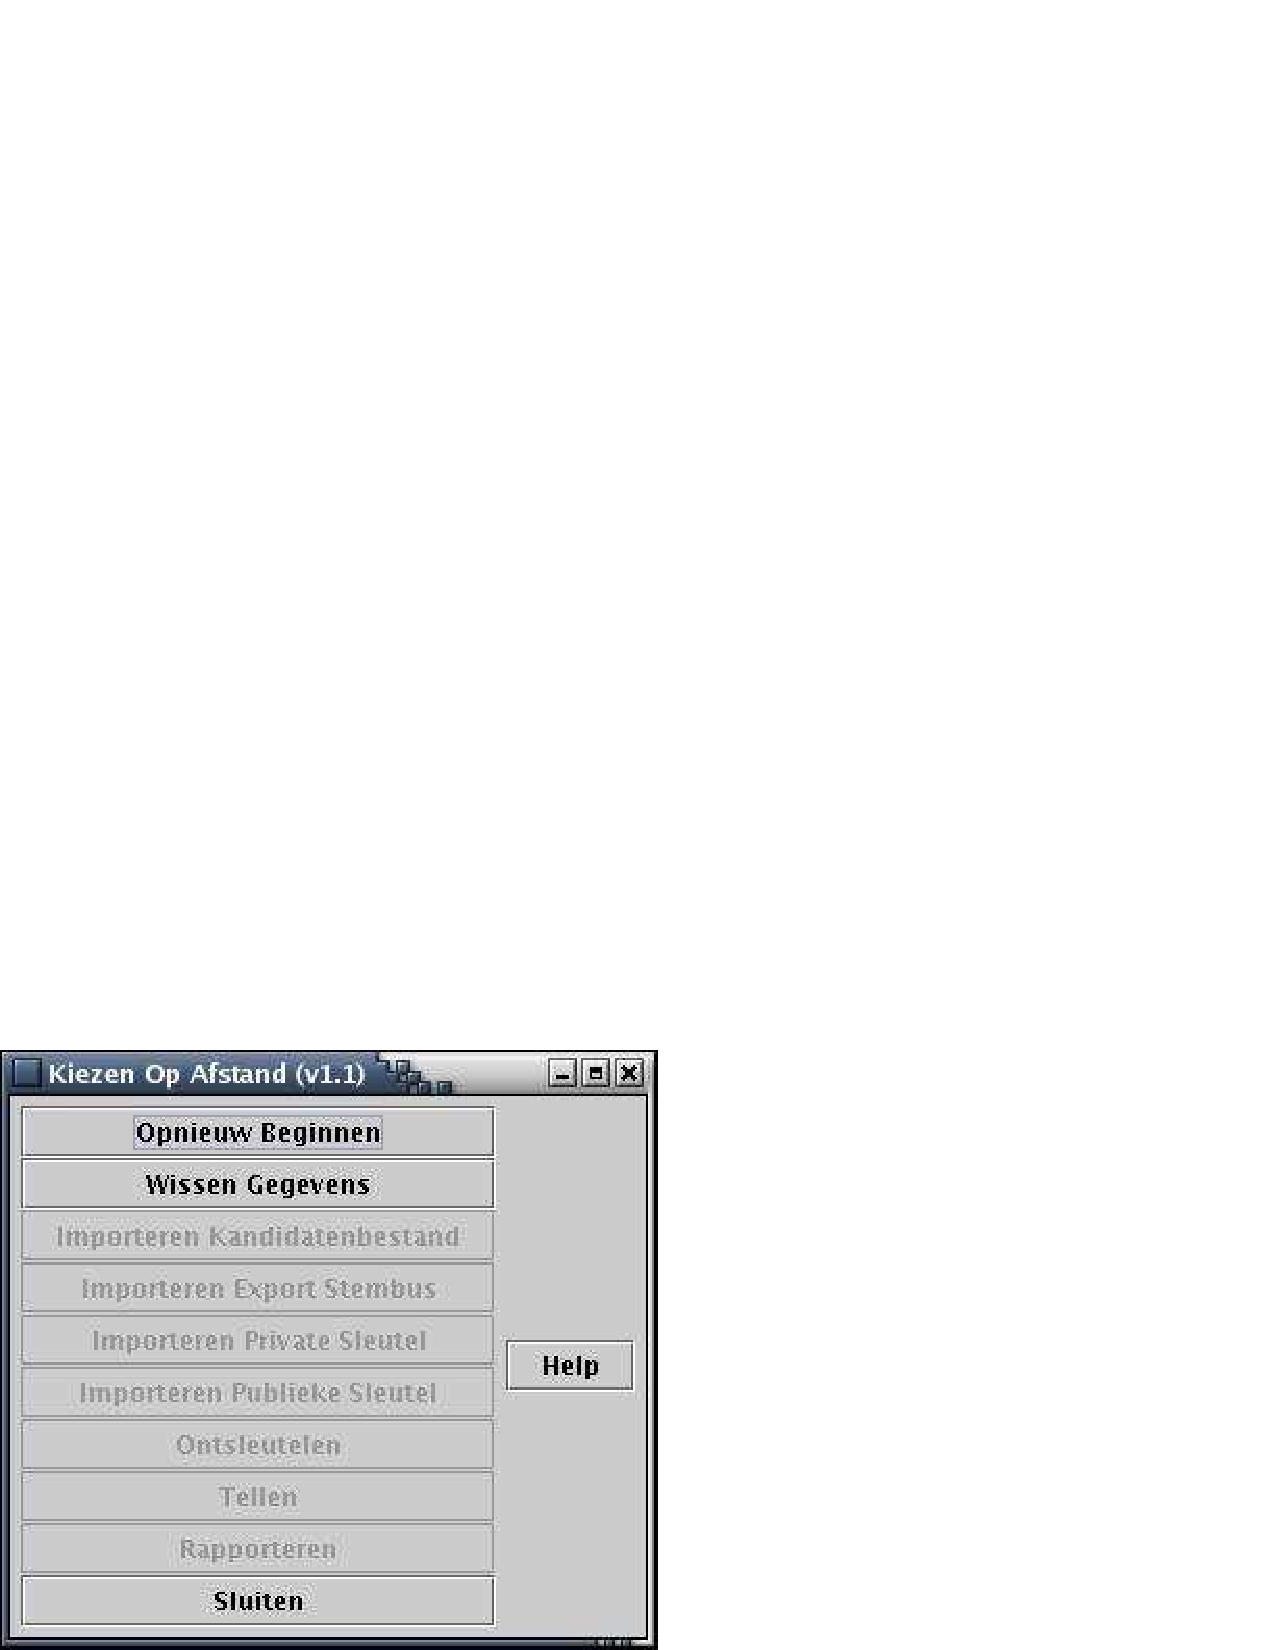
\includegraphics[scale=0.45]{scherm01}
    \else
    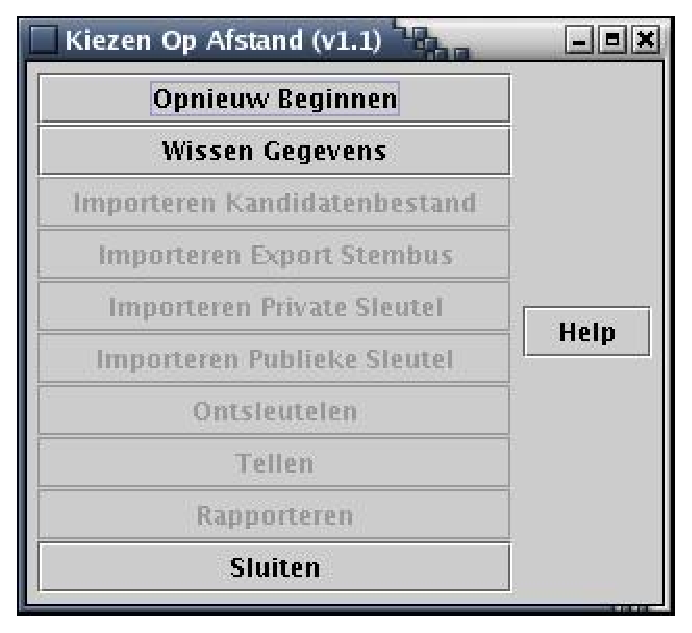
\includegraphics[scale=0.45]{scherm01.eps}
    \fi
    \caption{Het hoofdmenu direct na het opstarten}
    \label{fig:gui}
  \end{center}
\end{figure}
Het systeem om te garanderen dat de verschillende functies niet in een 
verkeerde volgorde kunnen worden uitgevoerd is direct te herleiden op
een toestandsdiagram waarbij de functies de toestandsovergangen zijn.
Zie figuur~\ref{fig:toestanden}.
\begin{figure}[htbp]
  \begin{center}
    \ifpdf
    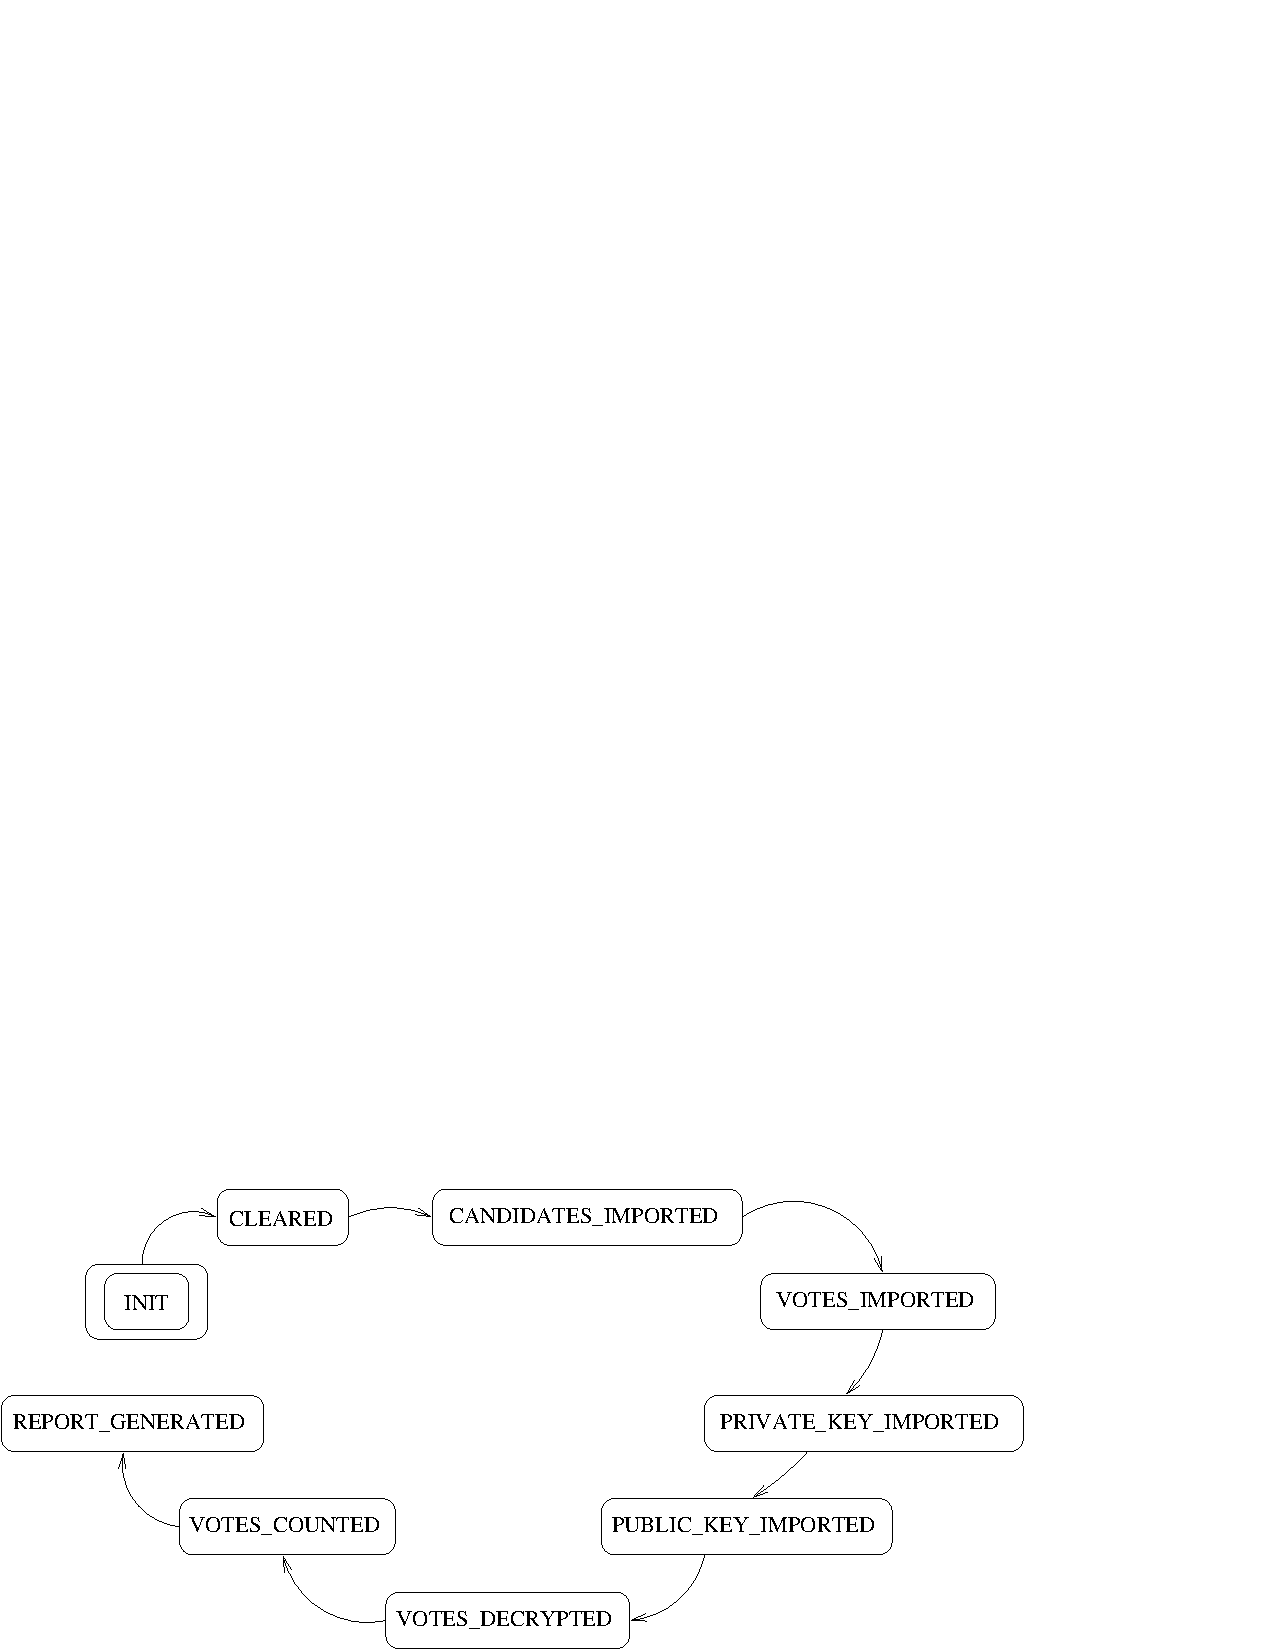
\includegraphics[width=80mm]{koa_state_diagram}
    \else
    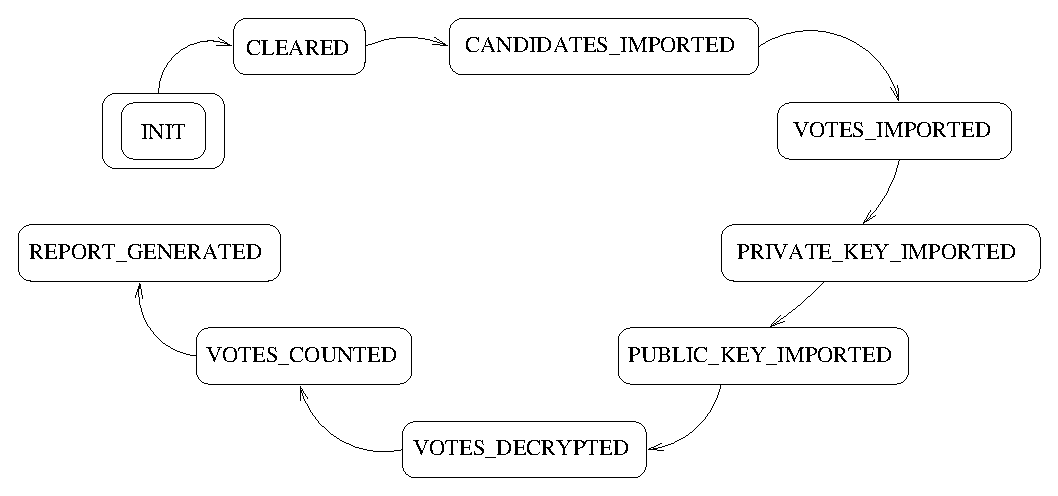
\includegraphics[width=80mm]{koa_state_diagram.eps}
    \fi
    \caption{KOA toestandsdiagram}
    \label{fig:toestanden}
  \end{center}
\end{figure}
Strikt genomen is deze automaat overigens niet volledig. Het is namelijk vanuit elke toestand toegestaan om weer opnieuw te beginnen. Deze transitie is niet wergegeven.

In \cite{Hubbers_Oostdijk_Poll:2003sec} wordt beschreven hoe zo'n automaat 
eenvoudig naar JML code kan worden vertaald.
In dit geval levert dat de code uit figuur~\ref{fig:guispec} op.
\begin{figure}[htbp]
  \begin{center}
    \begin{lstlisting}{}
/*@ spec_public */ int state; 

/*@ invariant state == INIT_STATE ||
  @   state == CLEARED_STATE ||
  @   state == CANDIDATES_IMPORTED_STATE ||
  @   state == VOTES_IMPORTED_STATE ||
  @   state == PRIVATE_KEY_IMPORTED_STATE ||
  @   state == PUBLIC_KEY_IMPORTED_STATE ||
  @   state == VOTES_DECRYPTED_STATE ||
  @   state == VOTES_COUNTED_STATE ||
  @   state == REPORT_GENERATED_STATE;
  */

/*@ constraint state == INIT_STATE ||
  @   state == \old(state) ||
  @   state == \old(state) + 1;
  */

    \end{lstlisting}
    \caption{KOA toestandsdiagram vertaald naar JML specificaties}
    \label{fig:toestandenspec}
  \end{center}
\end{figure}
In deze specificatie zien we drie verschillende dingen. Ten eerste wordt er een
normaal Java veld \texttt{state} gedefinieerd. Dit \texttt{private} veld
wordt \texttt{spec\_public} gemaakt om het mogelijk te maken om ook buiten
deze klasse over dit veld te kunnen redeneren.
Ten tweede zien we een invariant die niets anders is dan een opsomming van alle
mogelijke toestanden.
Ten derde zien we een constraint die aangeeft dat na elke methode aanroep
er moet gelden dat ofwel de applicatie weer in de begintoestand is, ofwel dat de toestand onveranderd is gebleven, ofwel dat de applicatie zich nu in precies \'e\'en toestand verder bevindt. Hierbij moet overigens worden opgemerkt dat de
waarden van de constanten natuurlijk zo zijn gekozen dat elke volgende toestand precies \'e\'en groter is dan de huidige toestand.

%%Helaas is zo'n constraint alleen nog niet sterk genoeg om te beschrijven wat er
%%precies gebeurt. Er is nu wel al gespecificeerd wat de mogelijke 
%%toestandsovergangen zijn, maar men wil natuurlijk graag ook nog vastleggen 
%%wanneer er gekozen wordt voor \'e\'en van de drie opties uit de constraint.
%%Dit wordt verder vastgelegd door de methode specificatie behorende bij de
%%gekozen functie. H'M DIT LIJKEN WE DUS HELEMAAL NIET TE DOEN...

Een belangrijke methode in het systeem is natuurlijk de methode waar het aantal
stemmen bij een kandidaat wordt opgehoogd. Het KOA systeem schrijft voor dat 
dit pas mag worden gedaan nadat er gecheckt is of de redundante informatie die
bij de kandidaatcode in de stem is opgeslagen overeenkomt met de informatie
behorende bij de kandidaat en de kieskring.
Nadat deze checks zijn uitgevoerd wordt de methode \texttt{addVote} uitgevoerd.
Zie figuur~\ref{fig:addvote}.
\begin{figure}[htbp]
  \begin{center}
    \begin{lstlisting}{}
  /**
   * Add a single vote to this vote set for the specified candidate
   * code.
   *
   * @param a_candidate_code the candidate code for which to increment
   * the vote count by one.
   * @exception IllegalArgumentException is thrown if the vote has not been
   * initialized or the vote has already been finalized.
   *
   * <pre><jml>
   * normal_behavior
   *   requires my_vote_has_been_initialized;
   *   requires !my_vote_has_been_finalized;
   *   requires 0 <= Integer.parseInt(a_candidate_code);
   *   requires validCandidate(a_candidate_code);
   *   assignable \everything;
   *   ensures my_candidate_list.getCandidate(a_candidate_code).voteCount() ==
   *           \old(my_candidate_list.getCandidate(a_candidate_code).voteCount() + 1);
   *   ensures my_candidate_list.getCandidate(a_candidate_code).kiesLijst().voteCount() ==
   *           \old(my_candidate_list.getCandidate(a_candidate_code).kiesLijst().voteCount() + 1);
   * also
   * exceptional_behavior
   *   requires !(my_vote_has_been_initialized &&
   *              !my_vote_has_been_finalized &&
   *              0 <= Integer.parseInt(a_candidate_code) &&
   *              validCandidate(a_candidate_code));
   *   assignable \nothing;
   *   signals (IllegalArgumentException) true;
   * </jml></pre>
   */
  final void addVote(final /*@ non_null @*/ String a_candidate_code) {
    if (!(my_vote_has_been_initialized &&
          !my_vote_has_been_finalized) &&
          0 <= Integer.parseInt(a_candidate_code) &&
          validCandidate(a_candidate_code)) {
      throw new IllegalArgumentException();
    }

    final Candidate candidate = my_candidate_list.getCandidate(a_candidate_code);
    assert (candidate != null);
    candidate.incrementVoteCount();
    candidate.kiesLijst().incrementVoteCount();
  }
    \end{lstlisting}
    \caption{\texttt{VoteSet.addVote}}
    \label{fig:addvote}
  \end{center}
\end{figure}
Ook in deze specificatie kunnen we weer enkele belangrijke aspecten zien.
Om te beginnen tonen wij hier hoe de JML annotaties automatisch binnen Javadoc
blokken kunnen worden weergegeven. Op deze manier wordt de specificatie zowel
door onze verificatie tools als door Javadoc gebruikt.

Verder zien we dat de methode specificatie uiteen valt in twee blokken: een blok\texttt{normal\_behavior} en een blok \texttt{exceptional\_behavior}.
Het eerste geeft aan dat de methode netjes termineert en de bijbehorende 
postcondities (\texttt{ensures}) zullen gelden bij de gegeven precondities (\texttt{requires}).
Het tweede blok geeft aan dat er een exceptie zal optreden bij de gegeven precondities. Hierna zullen de zogenaamde exceptionele 
postcondities (\texttt{signals}) gelden.

De eerste twee precondities van het \texttt{normal\_behavior} blok hebben te
maken met het specifieke datatype dat gebruikt wordt bij de stemming: om een
stem te kunnen toevoegen moet de stemming ge\"initialiseerd zijn en nog niet
afgesloten. De derde preconditie eist dat de ingevoerde string een niet
negatieve integer is. 
De vierde preconditie maakt gebruik van een andere methode. Die methode
checkt of er in de kandidatenlijst wel een kandidaat is die de opgegeven string
als kandidaatcode heeft.
Merk op dat het voor de tools niet uitmaakt of er \'e\'en \texttt{requires} wordt gebruikt waar een conjunctie van expressies achter staat of dat al die 
expressies een eigen \texttt{requires} keyword hebben gekregen. 
Het voordeel van splitsen is echter dat de tools nu duidelijker met een 
regelnummer kunnen aangeven welk deel van de totale preconditie nu precies
niet geldig was.

Als aan deze vier condities is voldaan zal de methode als reeds gezegd normaal
termineren. En zullen de twee postcondities moeten gelden.
De eerste specificeert dat het aantal stemmen bij de kandidaat met deze
kandidaatcode na afloop precies \'e\'en hoger is dan de waarde van diezelfde
methode bij het begin van de methode. Om onderscheid tussen de waarde van deze
variabele voor en na de methode te kunnen maken, gebruikt JML de \texttt{\\old}
constructie.
De tweede postconditie is bijna hetzelfde. Alleen wordt hier gesteld dat het
aantal stemmen van de partij waar deze kandidaat bij hoort ook precies \'e\'en
is verhoogd.

In het tweede blok staat als preconditie de ontkenning van de conjunctie
van de precondities van het eerste blok. Met andere woorden, deze twee blokken
zijn complementair.
De postconditie achter de \texttt{signals} is triviaal. Het gaat hier echter
om de \texttt{assignable \\nothing}. Dat wil zeggen dat er geen variabelen
gewijzigd zullen worden in dit geval.
In het bijzonder zullen er dus nergens stemmen bij een kandidaat of een partij
komen.

\bibliography{popular}
\bibliographystyle{alpha}
\end{document}
